\documentclass[a4paper,12pt]{report}
\usepackage[utf8]{inputenc}


\usepackage{graphicx}  
\usepackage{hyperref}
\usepackage{cite}
\usepackage{algorithm}
\usepackage{algpseudocode}
\usepackage{wrapfig}


\usepackage[font=normalsize,labelfont=bf, width=0.9\linewidth]{caption}

\usepackage{subcaption}	
%\usepackage{caption3} % load caption package kernel first
%    \DeclareCaptionOption{parskip}[]{} % disable "parskip" caption option
%    \usepackage[xsmall]{caption}

\setlength\fboxsep{0pt}
\setlength\fboxrule{0.5pt}

\setcounter{secnumdepth}{5}

\DeclareGraphicsExtensions{.pdf,.png,.jpg}
%\usepackage{cleveref}

%%%%% definition of custom commands %%%%%

% use when you need a ref to a section with hyperlinks like: ``section x, Section Name''
\def\sectionautorefname{Section}
\newcommand{\secref}[1]{\autoref{#1}}
%, \nameref{#1}
\newcommand{\And}{\textbf{ and }}
%\newcommand{\secref}[1]{\ref{#1}}

%%%%% end definition of custom commands %%%%%

%opening
\title{Rapid Geologic Modeling}
\author{Morten Bendiksen}

\begin{document}

\maketitle


\clearpage
\begin{abstract}
Drawing three dimensional models of geological phenomena is today a process requiring training in specific programs, and can be a time consuming process. For illustration and communication, geologists therefore often limit themselves to drawing on paper or in general two dimensional drawing programs on the computer.

In this thesis I propose an approach for making rapid geologic illustrations in 3D. The approach consists of sketch based input on and inside a cube, to create layers and other features. Awareness of the geologic domain enables relatively few input strokes to be interpreted. This awareness will speed up the drawing process and enable easier modification of the underlying model than in a generic modeling approach. A three dimensional geometry gives advantages like perspective control, lighting changes, etc.

I explore the relevant background material necessary and give a detailed description of the particulars of my approach and how it works. A user study was conducted with four geologists. I conclude based on this that the approach shows promise and can be useful in certain situations as it is now, and with further development could become even more useful.
\end{abstract}

\clearpage
\tableofcontents 



\clearpage

% --- OBS, gammel tekst i git commit 53adef7c5ef8730ab96a392efa1a10f1ae289f0b ---

\chapter{Introduction}
\label{sec:intro}


% --refer to each section at one point in introduction--\\
% 
% (present problem)\\
% 	- illustrations important
% 	- sketch 2d limiting\\
% 	- need tools for 3d modelling\\
% 	- existing 3d tools are advanced\\
% 	- need a simple/intuitive way to model\\
% 	
% (present goal)\\
% 	- replace paper and pen\\
% 	- not accurate/detailed\\
% 	- illustrative of ideas\\
% 	- for surveys or education\\
% 	- 
% 	
% (solution/approach)\\
% 	- the box metaphor\\\\
	

The earth is constantly changing. We have all experienced this through natural events such as earthquakes, volcanic eruptions, tsunamis, avalanches and floods. When we study such changes in a greater time frame, they are even more dramatic. In geologic time oceans are created and disappear, mountains are created and different forms of life go extinct and new life forms develop. Through much of human history big events like this were explained by appeal to the supernatural. The study of such changes is today the work of geologists. Geology as a science started in the 19th century, but is founded on scientific fields of inquiry much older that that.

Illustrations are important for geologists and their aspiring students when they are conducting their everyday business. It is normal to make sketched models by hand on either paper or computer. These are used in both professional and educational settings, and facilitate communication. On paper one is of course restricted to making two dimentional drawings. This can be limiting, since the fenomena of geology are of course three dimetional. One can sketch three dimentional fenomena by using perspective drawing techniques, but the model is still confined to the 2D nature of the medium. It is from this background that the goal of my thesis was formed; to create an approach for rapid and easy sketching of geologic structures in 3D.

On the computer it is already possible to make 3D models in many different ways. However, existing tools are often complex, aimed at creating advanced and detailed models, and usually requires training to understand and use. It would therefore be nice to have a possibility to make quick 3D models for illustrative purposes in a simple and intuitive way. This project has laid another brick in the foundation for the future of such illustrative geological modeling techniques. In the last section of the thesis (\secref{sec:conclusion}), I conclude that this has a large potential for use in education, for communication between geologists and in publications about geology, although more research is still needed.

This work presents an approach to rapid sketching of geological structures like rock layers, rivers, mountains and delta deposits. Geology is a vast field, and a lot of different features would be desirable to include. However, in order to finish, I had to limit the focus to the ones mentioned. The aim is to make a replacement for pen and paper 2D sketches of such structures. In other words, the aim is not a solution for situations where a high degree of accuracy is needed and/or attainable, but rather when the goal is to illustrate ideas and communicate them. In \secref{sec:eval} I therefore put the most emphasis on the expressive power the final solution gives the user relative to the effort needed, and less emphasis on accuracy. Resulting illustrations that were produced by users of an implementation of the approach can be seen in \secref{sec:results}.

It is in publications from the geologic feld I have found the most inspiration for this project. Artists in such media often use what I choose to call the ``box-model'' to illustrate concepts. Examples of such illustrations can be seen in \secref{sec:geology}. In that section we will also get an introduction to the relevant geologic background and terminology. Illustrations by geologists are often drawn inside a box cutout of the area of interest. This gives a good way to illustrate the spatial relation of elements in the model, like layers of different rock and deposits, rivers, ridges, mountains and the landscape they create together.

Illustrations using this ``box-model'' gave rise to the approach I have chosen. The user is initially presented with an empty box, and then proceeds by outlining on and in this box the particular features he wants to model. An explanation of the use of this technique and all others I have developed can be found in \secref{sec:concept}, while the algorithmic solutions are discussed in \secref{sec:method}. To put the work I have done in a scientific context I have included a brief report on the state of the art in the fields of Computer modeling and Geological modeling as they relate to this project, in \secref{sec:star}.
\clearpage


\chapter{Geologic Background}
\label{sec:geology}
\begin{wrapfigure}{r}{0.4\textwidth}
  \begin{center}
    \includegraphics[width=0.38\textwidth]{thesis/geo/core.png}
  \end{center}
  \caption{The structure of the earth.}
  \label{fig:core}
\end{wrapfigure}
This chapter gives a basic introduction of gological concepts. Focus is on those aspects that are needed to understand for the rest of the chapters in this thesis. The information that follows is based on the book ``Geologi, Stein, mineraler, fossiler og olje'', by Haakon Fossen \cite{fossen2008geologi}. 

Geology is a complex science, and this explains why there are so many fields within geology. Just a few of the fields will be mentioned here. Geomorphology is the study of landforms and the processes that shape the surface of the earth. Sedimentology is about how particles are transported, where they settle and are compressed into rock. Structural geology is the study of how the rock layers and crust is deformed by various movements. Tectonics is closely related to Structural geology and describes the movement of earth plates and how that causes the formation of mountain ranges and basins.

Geology is the study of the earth. The main purpose for the geologists work is to gain an understanding of the structure of the earth and the processes that shape it such as how mountains are built and how the oceans form. Most geologists usually concern themselves with only the surface and the part of the earth that is called the crust, the top 30 to 40 kilometers. Only rarely do they get into contact with what is deeper down. However, what happens there is still important to understand the processes that occur in the crust. 

Figure \ref{fig:core} depicts the structure of the earth. The core of the earth is over 4000 $^\circ$C. It is made up of an iron-nickel alloy. There is an inner core that is solid due to the high pressure, which raises the melting point, while the outer part of the core is liquid. Between the core and the upper parts, there is a thick layer called the mantle. The mantle has a malleable consistency like butter or dough, although it is less malleable the closer it gets to the core. It is thus able to move around without building tension and forming cracks. The upper part of the earth is called the lithosphere. It consists of the upper part of the mantle and the crust and it is stiff. This is why, when it moves around, it creates large amounts of tension resulting in earthquakes.

The earths crust is made up by several plates that are moving in relation to each other. They collide with each other, glide across each other, or separate from each other. Figure \ref{fig:fig99subduction} shows what happens at the point of contact and divergence.  Because of the large forces involved when the plates move around, the crust is constantly being changed by the plates being subdued underneath each other and made anew by magma flowing up at different locations around the earth at the place of divergence between the plates. The plates are not only made of the continents, but also consist of the oceanic crust and lithosphere. It is made at the points of divergence and is thinner and heavier than the continental crust. Therefor it floats lower in the mantle. At the point of impact, one of the plates is pushed down into the hot parts of the mantle, and melts away.

\begin{figure}
 \includegraphics[width=\linewidth]{thesis/geo/fig99subduction.png}
 \caption{Subduction and creation of oceanic plates}
 \label{fig:fig99subduction}
\end{figure}

Because the plates move around, large tensions can build up in them. When the tension gets bigger than what the rock can withstand various structures will appear. Such structures can occur where the plates meet, split apart and glide across each other. They can also occur in other places where tension might build. A layer of rock might fold, get stretched or break apart. Different types of rock might react differently to tensions according to their mineral composition and the temperature when the deformation occurs. When rock reacts by breaking apart, fractures are created. There are two types of fractures, faults and cracks. Cracks have very little movement along the fracture direction, and occur all over the earth. They can form when rock is lifted and compacts due to the falling temperatures. Faults are fractures where there has been considerable movement along the fracture direction. Figure \ref{fig:faults} shows different types of faults that can occur. In stead of breaking apart and creating a fault, the rock might also fold, bend and stretch, creating a shear zone. They look similar to faults, but are wider, and in stead of the discontinuity of the broken rock have a zone where the rock is folded and stretched along the movements direction. Such shear zones are created in warm and deep parts of the crust, where rock becomes softer.

\begin{wrapfigure}{l}{0.4\textwidth}

  \begin{center}
    \includegraphics[width=0.38\textwidth]{thesis/geo/faults.png}
  \end{center}
 
  \caption{Different types of faults}
  \vspace{15pt}
  \label{fig:faults}
  
\end{wrapfigure}

In the deep it is also normal for rock layers to fold. Folds are very frequent in metamorphic rock types. One way normal folds are created are by compression of layers, where the forces are working in the direction of the layers. Another way is by shearing movement. However, folds can also occur nearer to the surface, especially in sediments that have yet to complete it's transition to firm rock.

\begin{wrapfigure}{r}{0.4\textwidth}
  \begin{center}
    \includegraphics[width=0.38\textwidth]{thesis/geo/fold.png}
  \end{center}
  \caption{Folded rock}
  \label{fig:fold}
  
\end{wrapfigure}

The age of the earth is about 4.6 billion years. Geologic processes that shape it take a very long time and still continue today. Geologists need to understand what processes took place during this time, how geologic phenomena have and is still interacting with each other over time, and how structures that can be observed, relate to each other in the geologic time scale. Often layers can be observed to be stacked neatly on top of each other in which case it is easy to understand that the youngest layers are on top of the older ones and a relative time scale can thus be mapped for these structures by simple observation. Even when layers have been distorted, an understanding of the processes involved makes it possible to establish such a relative time scale. By radiometric dating, on the other hand, one can establish an absolute time scale. This is possible by studying the decay time of radioactive materials. This makes it easier to relate different structures around the world in a time scale.

The geologic time scale, as illustrated in Figure \ref{fig:geoTime}, has been developed by studying layer structures around the earth and dating them. The scale shows the relative times of different processes, but also as radiometric measurements of the different structures have been taken it has become possible to date the events that created them absolutely. In a similar way to how a historic time scale can be divided into stone age, bronze age, iron age, middle age and so on, the history of the earth is also divided into eras and time periods. The closer we get to our own time, the more details are known and included in the geologic time scale. Fossil records also give useful information about the relation and absolute position in time of structure found at different places, without having to do a radiometric dating every time.

\begin{figure}
 \includegraphics[width=\linewidth]{thesis/geo/geoTime.png}
 \caption{The geologic time scale}
 \label{fig:geoTime}
\end{figure}

\begin{figure}[]
        \centering
        \begin{subfigure}[b]{0.3\textwidth}
                \centering
                \includegraphics[width=\textwidth]{thesis/geo/gabbro.jpg}
                \caption{Igneous rock (Gabbro)}
                \label{fig:gull}
        \end{subfigure}%
        ~ %add desired spacing between images, e. g. ~, \quad, \qquad etc. 
          %(or a blank line to force the subfigure onto a new line)
        \begin{subfigure}[b]{0.3\textwidth}
                \centering
                \includegraphics[width=\textwidth]{thesis/geo/sandstone.jpg}
                \caption{Depositional rock (Sandstone)}
                \label{fig:tiger}
        \end{subfigure}
        ~ %add desired spacing between images, e. g. ~, \quad, \qquad etc. 
          %(or a blank line to force the subfigure onto a new line)
        \begin{subfigure}[b]{0.3\textwidth}
                \centering
                \includegraphics[width=\textwidth]{thesis/geo/quartzite.jpg}
                \caption{Metamorphic rock (Quartzite)}
                \label{fig:mouse}
        \end{subfigure}
        \caption{Pictures of rock types}\label{fig:rocks}
\end{figure}

If we disregard water, vegetation and dirt, the surface of the earth is made of rock. Rocks are made out of different minerals and come in many different varieties. Minerals are chemical elements bound together in certain ways. For a compound to be called a mineral it must be solid, have a particular chemical composition and a special crystalline structure. The mineral composition of rock is an important aspect that geologists study when examining geologic structures. There are three types of rock. Igneous rock, sedimentary rock and metamorphic rock. Igneous rock forms when magma (molten rock) crystallizes into solid form. When this happens in the deep where the temperature is high, crystals have long time to form. When crystal forms slowly like that, the individual crystal forms become bigger than when they are rapidly cooled down. If the magma reaches the surface before it crystallizes, we get smaller crystal forms, and thus a more fine grained rock. Sedimentary rock forms when sediments like clay, sand and gravel is transported and deposited over time and solidifies into rock after it settles. Sedimentary rock cover about 75\% of the continents of the earth. When either igneous or sedimentary rock gets under high pressure and temperature, they start to change their mineral composition and deformation. They then become what is called metamorphic rock.

\begin{wrapfigure}{l}{0.6\textwidth}
  \begin{center}
    \includegraphics[width=0.58\textwidth]{thesis/geo/geoDeposit.png}
  \end{center}
  \caption{Different processes that deposit sediments}
  \label{fig:geoDeposit}
\end{wrapfigure}


Figure \ref{fig:geoDeposit} shows many of the processes that can erode rock and deposit material elsewhere. The study of erosion, deposition and how this creates sedimentary rock structures is the most important way geologists have developed scientific knowledge about the history of the earth. When rock is exposed to the weather it is eroded away and becomes loose particles of clay, sand or gravel. It is transported by water, wind or ice until it settles at some other location. These forces are constantly trying to flatten the features of the earth. Mountains are eroded away, while basins and valleys are constantly being filled with material. All the different processes that deposit material will create layers of different kinds of sedimentary rock. These layers are called strata. Figure \ref{fig:strata} shows such strata once created in a delta system by a river.


\begin{figure}
 \includegraphics[width=\linewidth]{thesis/geo/strata.png}
 \caption{Delta deposits in Book Cliffs, Utah. The deposits have formed layers, or strata of different rock types.}
 \label{fig:strata}
\end{figure}

Rivers will form from precipitation, and as they run trough the terrain will dig out and erode it, while at the same time transporting material downstream. This creates valleys in the terrain where the river runs in the bottom. As the river digs out the terrain it creates a v-shaped valley, more pronounced farther up the river, and considerably wider at the bottom. As the river carves lower, parts of the valley sides will also start falling down, also widening it. In the lower parts, the river will at some point not be digging out any more, but rather only deposit material from the upper parts thus flattening the landscape over a long time. Rivers can flow in different patterns.
\begin{wrapfigure}{r}{0.5\textwidth}
  \begin{center}
   \vspace{-15pt}
    \includegraphics[width=0.48\textwidth]{thesis/geo/miss.jpg}
  \end{center}
   \vspace{-15pt}
  \caption{The Mississippi river delta}
   \vspace{10pt}
  \label{fig:miss}
\end{wrapfigure}
Where the terrain is steep, they will flow more straight and where there is enough water they can flow in a braided pattern covering a large area. If the terrain is flatter rivers usually follow a meandering pattern, flowing back and forth in meanders. Meandering rivers dig in the outer sides of meanders and deposit in the inner side of meanders. Thus they will move around in the valley where they flow. Sometimes a meander get cut of, leaving an abandoned meander. 


Where the river meets the sea, it will create a delta deposit system. A delta is formed by the deposition of sediments carried by the river. Since the river is no longer confined to it's valley the flow will spread out and the flow velocity will drop. This means that the flow can no longer carry sediments, and they will deposit. As sediments are carried out into the sea, they tend to create s shaped deposits called clinoforms which can build outward into the sea. As the river deposits material, the slope of the river will therefore decrease as it builds outward in the sea. As the slope decreases the river path will tend to get unstable, and the river finds a new way to reach the sea after a while. In this way the river path changes and distributes the deposits. The delta can take many forms depending on the circumstances. Figure \ref{fig:delta} shows the structure of a possible delta system. Figure \ref{fig:miss} show a picture of the Mississippi river delta.





\begin{wrapfigure}{r}{0.35\textwidth}
  \begin{center}
   \vspace{-15pt}
    \includegraphics[width=0.33\textwidth]{thesis/geo/coal.png}
  \end{center}
   \vspace{-15pt}
  \caption{Making of coal}
   \vspace{-15pt}
  \label{fig:coal}
\end{wrapfigure}
When looking for resources, many different insights from the different fields of geology are important. Coal, oil and gas are examples of very important resources where all necessary knowledge is used to make the search and recovery efficient. Figure \ref{fig:coal} shows how coal is formed from biological material being compressed and heated. When it is buried, gases and liquids are forced out, and chemical reactions happen. As time passes the carbon content in the coal rises.




Oil and gas is formed from organic material like plankton and algae that is buried without access to oxygen. It takes millions of years to develop when there is the right temperature. Figure \ref{fig:oilMigrate} shows how, when it is mature, the oil and gas will migrate upwards. If it hits certain structures in the rocks layers it can get get stuck there. Such areas are known as oil traps. The study of geologic layers can therefore help in determining where oil and gas can be found. When looking for such resources, very often a seismic study will be made. Simply explained, this consists of sending sound waves down into the rock and listening for the echoes. At the boundaries of layers some of the sound will be reflected. By recording how much time it takes for each reflection, and by repeating this procedure at different locations, it is possible to create images of the horizons underneath the surface. Another technique for gathering data on the subsurface is by boring holes and taking physical samples or measuring other properties of the rock directly. Interpreting the data that is is one of the jobs geologists do to determine where resources might be found. Many technologies exist to help geologists do this interpretation to create a model of the subsurface.

In this chapter we have seen many different illustrations of geological structures. Geologists frequently need to make such illustrations and models of what they are researching. Geological modeling tools is one of the things that are described in the next chapter, which outlines the state of the art of computer and geological modeling.
%\begin{wrapfigure}{r}{0.35\textwidth}
 \begin{figure}
  
 \begin{center}
    \includegraphics[width=0.33\textwidth]{thesis/geo/oilMigrate.png}
  \end{center}
  \caption{Migration and trapping of oil and gas}
  \label{fig:oilMigrate}
 \end{figure}

%\end{wrapfigure}

% Figurer
%  12.7, 

% Include detailed explanation of different processes of deposition

\clearpage
\chapter{Related Work}
\label{sec:star}

This chapter explores the field of 3D computer modeling as it applies to geologic modeling with special focus on techniques for rapid modeling. 3D models can be made in many ways, they can be made manually, automatically, or with a combination of both.  A traditional way to create 3D models on the computer called computer-aided design or CAD, usually consists of modeling and compositing different kinds of solid objects to create precise models of industrial designs, buildings etc. One commercial program of that type is Autodesk AutoCAD. Other types of 3D modeling consists of editing vertices and control points of curves, which are often used for movies, games and other graphics purposes. A commercial example of that is Autodesk 3D Studio Max.

Models can also be represented in various ways. Many modeling programs use a polygonal representation, meaning 3D vertices, connected by edges, forming polygons. These are easy to visualize and manipulate for the computer hardware.  Others use a mathematical representation of solid objects. There are well established ways to create detailed and sophisticated 3D models with these representations. A lot of research has been done on this type of modeling over the years and much progress has been made. However, it still requires a substantial amount of training and the modeling often takes quite a bit of time. When creating models that do not need to be perfect, such as rapid prototyping models, illustrative models, models for communication etc. this can be prohibitive. Therefore a lot of research has gone into developing alternative methods for user input for enabling more rapid 3D modeling in recent years.

%\section{Rapid 3D Modeling}
 Sketch based input is one way of achieving simpler and more rapid modeling input. With sketch based input the idea is to do 3D modeling with a method that is made to feel more like traditional pen and paper sketching as opposed to editing vertices and edges directly.
The SKETCH system was one early development in this area \cite{zeleznik2007sketch}. With SKETH, Zeleznik et al. produced a gesture-based input method for rapid modeling of simple 3D geometric shapes that could be composited using constructive solid geometry (CSG). Teddy \cite{Igarashi:1999:TSI:311535.311602} later expanded on these ideas by creating a freeform sketching tool for 3d models where the user draws the silhouette of objects, and they are created automatically. Teddy made it simple for even first time users to make simple, expressive figures. A Brazil et al. \cite{brazil2010sketching} also show promising results for modeling soft looking objects by sketching variational hermite-RBF implicits.
Digital sculpting is an alternative method of input for easing 3D modeling, where the modeling more resembles real world sculpting by applying pressure and similar methaphors. Z Brush by Pixologic is a modeling program that uses this approach.
 

%\section{Geologic Modeling}
In geology, models are used for understanding and communicating about phenomena relating to the structure of the earth and how it changes over time. Most existing tools are based on the assumption that there is extensive data available and that geologists will have a lot of time developing a model of the area of interest. Several tools exist for modeling, displaying, editing and automatically calculate parameters for geological modeling.  Petrel \cite{petrel} is an example of a commercial programs for geologic modeling that is in use. Most of such existing tools rely on an intensive work flow, and are based on interpreting data gathered from seismic surveys or bore hole data. The modeling is done either automatically, or semi-automatically by letting the user indicate various parameters and alter the suggested model manually. Sometimes up to a year is spent on developing such models. Recently a need for rapid developments of geologic prospects have been identified. In such cases a model must be made more quickly. A lot of techniques have therefore been taken from other fields that model terrain, such as the video games industry and movie industry.

Natali et al. explores different modeling techniques in their recent report \cite{natali2013modeling}, which has been approved for publishing. They describe a data oriented taxonomy where modeling is divided into three different scenarios, one data free, one data sparse, and one data dense. They also describe a workflow oriented taxonomy, where modeling is divided into the separate stages necessary for creating a geological model. They also show how geological modeling trends are approaching modeling methods that have been developed in computer graphics. They also have an in-depth description of selected methods for geological modeling.

The data free scenario is the one this thesis concerns itself with, since the idea is to create a sketching tool, as explained in the introduction. However, some aspects from the other scenarios are also relevant here. The data sparse scenario is the most normal one in the geoscienses and is most often the result of borehole data. 
 The data points are spread around and needs to be interpolated.
 The main interpolating methods are the B-Spline method, inverse distance method, Kriging method, and discrete smooth interpolation method \cite{Mal92, Mal97}.
 The data dense scenario is usually when data from seismic surveys is available. Here the problem is how to display the huge amounts of data, and how to interpret them to make a model of the structures present. Patel et al. describe techniques for rapid horizon extraction in both 2D \cite{PGT*08} and 3D \cite{PBVG10}. The data free scenario has no ground truth information and relies entirely on procedural and geometric modeling. 
 
 Procedural generation of terrains usually happens in one of three ways: fractal landscape modeling, physical erosion simulation and synthesis of terrain from images or sample terrain. Before Olsen \cite{Ols04} fractal noise was mostly used to create terrain surfaces, because of computer limitations on simulating erosion processes. Olsen proposed a synthesized fractal terrain and applies an erosion algorithm on that. The representation is a 2D height-map. 
 
 

Turner \cite{turner2007review}

A geological geological scenario follows certain constraint. Caumron et al. \cite{turner2006challenges} gives rules for modeling that define boundaries between layers. For example, geological objects have a spacial continuity such that abrupt changes of normal orientation are not common. They also describe  the typical process of creating a structural model. The modeling usually starts with fault modeling, then the connection between fault surfaces is defined. Finally horizons are modeled. If the fault structure is very complex, it is normal to start with horizon definition and introduce the faults after.

Not that many purely sketch based input methods exist for the geology domain that I could find. Natali et al. \cite{natalirapid} describes an approach where the user sketches the boundaries of geological layers on a 2D vertical plane. Then the user can sketch folding and faulting operations, and thus create many different scenarios. The input in this approach is restricted to making conceptually 2D sketches, allthough the visualization is in 3D. Projecting drawings on the 3D structure can however give some more information and context than a pure 2D approach. Amorim et al. \cite{amorim2012sketch} descibe how various sketh based approaches can be used to allows the user to sketch directly over the raw seismic reflection volume and its derived data. This helps the expert in interpreting and and building a structural framwork for a reservior by using a sketch based input for helping in the interpretation process.

There exists several approaches for sketching terrain, which are applicable to geology. Harold is an early example of a sketch based system that incorporates methods for sketching terrain, made by Cohen et al. \cite{cohen2000harold}. In Harold, the user can sketch hills on the terrain by simple strokes that start and end on the terrain. The terrain is then warped to try and match the stroke. Watanabe et al. made a further development of this in \cite{Watanabe:2004:SIT:1186415.1186500}, where the shape of the stroke also influences the width of hills that are generated, making for more natural looking hills. They also incorporated noise on top of the generated terrain to make the visualization more realistic. Gain et al. later improved further on this by allowing the user to sketch the width of the hill and change the baseline along wich this hill runs \cite{Gain:2009:TS:1507149.1507155}.

Some geologic modeling tools exist for educational purposes that allow the realatively rapid building of geological phenomena by inputting various paraters. Cockett's Visual Geology \cite{Cockett:Online} and Jessell's Noddy \cite{jessell1981noddy} are two such programs. Visual Geometry lets the user specify things like how many layers he wants ant their thickness, and then apply various functions like a fault line and it's angle, a folding phenomenon and it's angle, wave frequency etc. The basis for Noddy is the ability to construct a complex geological history as a succession of relatively simple structural, sedimentary and igneous events similarly to Visual Geometry, which allows you to rapidly create models and then calculate resulting gravity and magnetic fields.

\clearpage



\chapter{Work process}
This chapter describes the research and development process from start to finish. It begins by explaining how the first idea was formed and how the initial research proceeded. The next section regards how collaboration with geologists and students helped the progression of the project. The chapter ends by describing the development of the approach itself.
\label{subsec:work}
\section{Inspiration and research}
As mentioned in \secref{sec:intro}, work started with the need for a tool to rapidly create three dimensional sketches for geological structures. Various existing geological illustrations were investigated and there were some discussions about what would be the goal. At the beginning however, there was not a clear idea of to approach it or how this would be achieved. Research therefore started by reading some geologic papers and books, both to get an idea of what kinds of sketches was needed, what was to actually be sketched and to get a litte bit of an overview of what geology is.

A large portion of the sketches encountered in litterature were drawn inside a cube shaped cutout. The cutout of the geologic structure along a primitive and easy to understand object like a cube, gives the viewer a good way of understanding how the different structures relate to each other. This was how the idea of the sketch cube, which is the starting point of the approach presented in this thesis, began.

To make a final decision to proceed with that approach, a more detailed strategy was needed. Therefore a new research phase began, were techniques dealing specifically with sketch based input, procedural modeling, terrain modeling, geological modeling etc. were researched. A couple of example illustrations that were found in a geological research paper \cite{neal1993sequence}, were used as a goal for what was to be possible in the program. Figure \ref{fig:inspiration1} these illustrations, which depict several depositional rock layers at the different times when they were deposited. The sea level at which they were deposited is indicated by the dotted lines. A set of different geological phenomena could be seen in these examples. Further research of modeling techniques gave some possible ways to do the input of such features, An idea of how the finished solution could look and function from a users perspective was forming.

% TODO give examples of the techniques mentioned

\begin{figure}
 \includegraphics[width=\linewidth]{thesis/inspiration1.png}
 \caption{Example illustration that served as inspiration in the beginning of research. Image from Sequence Stratigraphy - A Global Theory For Local Success, by Neal et. al}
 \label{fig:inspiration1}
\end{figure}


% TODO add description to appendices
to explain the idea, illustrations and explaining text were put in a project description document. Figure \ref{fig:riverDesription} is an example illustration from that document showing how drawing of river structures was planned. The complete document can be found in the appendices. This was the basis for the implementation work at the beginning of the project. A lot of further research and clarification of ideas was still needed, but since the general approach had been decided, the only thing remaining before development of a concrete approach could begin was to decide on technology.

\begin{figure}
 \includegraphics[width=\linewidth]{thesis/river.png}
 \caption{Illustration of how the drawing on rivers were planned to work at the beginning of the project, before implementation started. First, drawing a line on a surface where the rivers should go. Then, a river is created by an algorith in the program}
 \label{fig:riverDesription}
\end{figure}


\section{Collaboration}
After having created a version of the program that could be used as a prototype for demonstration, a professor from the department of geology was contacted. He also put me in contact with a geology student. The rest of research and development was guided by the collaboration with them. 

The basic idea of the solution was shown to a professor of geology. He showed great interest and believed this could be good approach for illustrations in geology and he had some suggestions for improvements. What what learned from this meeting was that the focus on the ability of creating nice looking sketches rapidly was the most important. There were also some other ideas and features suggested for further development. These included things like illustrating the sea level, illustrating vegetation and many more ideas. Features that I had already thought of, like mountains and rivers, were confirmed to be important also. To help assess the development and suggest more improvements in the future, he gave the contact details of one of his students, Marie Songve.

%%%%%% TODO append notes from meeting

Marie helped develop some paper sketches that would be the main focus of development( see sketch in Figure \ref{fig:illuSketch} ) from that point on. She also helped assess and guide the development through the rest of the implementation phase. In addition to giving concrete advice on the geologic features of the program, observing the usage helped identify the biggest user interface problems. After implementation Marie also helped in assessing the success of the project by giving her impressions and trying out the program by creating several sketches on her own. The results of this can be found in \secref{sec:results}. The collaboration with geologists was very helpful in guiding development direction and in taking choices during the implementation.


\begin{figure}
 \centering
\includegraphics[width=.4\linewidth]{thesis/illuSketch1.png}
\includegraphics[width=.4\linewidth]{thesis/illuSketch2.png}
 \caption{Reproduction of hand made sketches that were made in collaboration with Marie Songve}
 \label{fig:illuSketch}
\end{figure}

\section{Implementation work}

In this part the progression of work will be explained without going into much detail about the specific solutions created. The Only details included are those that are relevant for understading the most important choices which are discussed here and which are not explained earlier. For more details about the specific solutions, have a look at \secref{subsec:indepth}.

Implementation work was started by creating the cube and a camera system that would allow rotating around and zooming in and out of the cube. This was achieved relatively quickly. Intersection tests and input on the cube was the next step. At first this was achieved by simply looping through all the triangles and storing each intersection point in a list, and then drawing lines between the points that were drawn. However, the next step was the real challenge, which had not really been considered in depth until now. That challenge was how in the world to create a sensible layer from lines drawn on the faces of the cube. Different approaches were tried, and the details of how that turned out can be found in \secref{subsec:layers} further back. This ended up taking a lot more time that was initially expected. However, in order to focus on the solution, one has to know the problem, so all the work that might seem like a waste was actually needed in order to realize that there was a problem and therefore what 
kind of solution to look for.

Once a solution to the layer problem was found, there was of course a lot of other features needed to create a program that could be used for making useful sketches. Meetings with Marie helped focus the direction and prioritazation of their implementation. All the different features that were planned in order to reproduce the initial pen and paper sketch, were going to be implemented one after the other. Very often introduction of new capabilities meant going back and modifying existing code. In addition there were the non-geologic features of the program to think about, like undo functionality, save and load possibilities etc. These also had to work togheter with the other features in a way that would not upset any of the other features. As new features were added, it sometimes seemed as if the complexity was growing exponentially. It quickly became a problem keeping the different features working together in a smooth and predictable way. The program code was therefore changed many times to try and abstract 
the complexity to make the implementation of new features as easy as possible.

It was while realizing the complexity of the initial approaches that an idea of a parametric and ordered hierachical structure was introduced. In the start, everything was based on three dimentional coordinates, which made it difficult to calculate the relationship between for example the points on a layer and a river on it. If the layer changed, what point on the new surface would correspond to the beginning of the river? The user would have to draw the river again, which was not a good solution for a rapid modeling tool. The idea was that parametric coordinates would restrict the placement of a feature to two dimensions on it's parents surface. Thus, a new point in three dimentions could be calculated based on the parents position and geometry. The inspiration for this approach came from the paper by Schmidt et al. \cite{CGF:CGF1129}. This would ease the recalculation of coordinates once something changed. The ordered structure meant that each feature would only have to deal with immediate parent and 
children, and the order in which they had been drawn would be the guiding way to solve conflicts that might arise. The thought behind this was that the user would be thinking of the structures in a hierachical way already, and after familiarizing himself with the program would know in what order features need to be drawn to create the desired effect. After all, it does not make sense to have a river without first having a surface on which it flows.

The parametric and hierachical solution could now be used for many problems. For example, how does one specify the height of a ridge and how does this height change if the layer changes, and how and where does it affect the underlying parent? The simple solution was making the ridge baseline a parametric coordinate on the layer, and for each point along the baseline, there was associated a height value, which could then be used to compute the actual resulting top point of the ridge by first finding the position of the baseline point on the surface, and then adding the height. How to do the actual morphing of the underlying surface to create the ridge also became a lot easier, since the lookup of surrounding points now was restricted to two dimentions and the baseline point was already known in this space.

There were of course a lot of other difficulties remaining to solve to reach the stage the program is in now. However, the rest of the development was more about smaller issues local to each problem, and will be covered in the relevant subsection in \ref{subsec:indepth}.  There were still complexity issues of course, about how to fit each feature into the general solution without interfering with what was already implemented. New ideas were developed as work progressed, and others discarded along the way, mainly for lack of time. Going into all those details would mean we could write several books, but the details about solutions that have been implemented, and the problems and their solutions that are relevant to understanding choices will be included in the next two sections.


\clearpage


\chapter{Methodology}
\label{sec:method}
This chapter starts by giving an introduction and overview of the solution in \secref{sec:concept}. We provide an explanation of the approach and provide an introduction to the general solution and possibilities. We also provide a brief introduction to the different features  that are in the final approach. This will help set the context for the rest of the chapter.

We proceed with \secref{subsec:work}, by taking a look at how the work was planned and how it progressed, from definition, through research and development, to the final solution. 

\secref{subsec:generaldesign} provides an explanation of the design, i.e. how algorithms and data structures are used throughout the solution, without going into the details of specific solutions. We explore how they work together to enable the drawing of sketches from input to finished model at a conceptual level. This part is intended to give an overview of how the algorithms work.

 We then present a more detailed view of the specific features of the program in \secref{subsec:indepth}. Here we focus both on why different decisions about design were made, and provide an in-depth presentation of the algorithms. Each feature is illustrated with example screenshots.

The chapter concludes with \secref{sec:tech} by describing what technology like programming language was used and how other supporting features like save and load were realized.

\pagebreak

\section{Basic Concept}
\label{sec:concept}

\begin{figure}[h]
 \includegraphics[width=\linewidth]{thesis/overviewConcept.pdf}
 \caption{Conceptual overview}
 \label{fig:overviewConcept}
\end{figure}

Figure \ref{fig:overviewConcept} gives a conceptual overview of the approach. The arrows represent processes, either in the computer or performed by the user. the Square boxes represent data. The user starts with an idea in his head of what he wants to model. He indicates what he wants to create through input using the mouse, resulting in the input data. The program interprets the input data, and for each feature recognized, creates a representation of it in the scene tree. The representation is then used by the geometry synthesis code, to create new geometry and alter the shape of existing geometry.This happens at interactive frame rates. Once the scene geometry is ready, it is used by the visualization code for creating an image that is given back to the user on the computer display. The user then compares what he sees with what he had in mind. He can then do further refinement of the model by either changing some of what he already drew, or adding new features by drawing on the existing geometry.

The basic idea of the approach, is based on a cube on which the user will draw curves that represent an outline of a surface. The cube can be viewed from all directions by means of a virtual camera that rotates around the scene. These surfaces represent the horizons of geological layers that could represent the strata of depositional rocks or other layered structures. By further sketching or user input it is then possible to modify these layers to create other structures like rivers and ridges. For the rest of the text, such structures that can be made by the user are called features. Most of the input consists of drawing simple curves on surfaces, and then indicate what kind of feature is wanted. However, it was an idea from early on in the project to see if it would be possible to make a combination of a sketching approach to modeling with a procedural approach. By procedural I mean that the geometry is calculated by some algorithm in stead of the user sketching it or in other ways specifying it's final geometric properties. A feature for creating depositional delta structures has been implemented procedurally. A deposit in the current approach is a layer of material that has been deposited by a river where it enters the sea. The geological background chapter explained how all sedimentary rock layers are created by such deposited material. All features are created based on the users input, meaning that there is no data representing real world conditions given as input to the algorithms.

The users input has to be interpreted in some way. The most significant part of the input is the selecting of geometric structures in the scene, and drawing of curves on these structures. The first part of this process is to transform the screen space coordinates of the mouse into a ray pointing into the scene from the position of the camera. This vector is then used to check for intersections with the geometrical structures in the scene. Depending on which mouse button is pressed, the feature that the geometric structure belongs to is either marked as selected, or the point of intersection is added to a structure representing a curve that is visualized to the user. Some special interpretation rules are in place for different features which will be covered later. By clicking on various buttons in the user interface, the user provides information of what his input was intended to represent.

Once this basic input has been gathered the intent of the user understood, each of the features does further interpretation of the curves that have been drawn. The output is an internal representation of the model. The internal representation is contained in a tree structure where the cube is always the starting point.  Every feature added will add a new node in the tree. This internal representation does not store the 3D points where the user drew in the scene, but rather uses a 2D parametric representation. Each 3D point can be found by looking up it's placement by a function defined in the parent feature. This internal representation is used later in the process to compute a 3D geometry based on triangles, which can then be visualized on the computers screen via the graphics card. The user will utilize this generated geometry as visual feedback, and decide whether it is close to what he intended, or whether he needs to give additional input or change his input to achieve what he wants. Thus the process continues until a satisfactory result has been reached. Now, the user can store the work for later, send it to someone else, or take screenshots for use in a paper, lecture etc.




The purpose of the internal representation is to capture the modeler's intent as well as possible. From a technical viewpoint, it is the the meaning of the input that is interesting and stored for the representation. How the geometry is presented in the end is interesting for the user, but capturing the intent enables a modeling approach that lets the user to go back and change earlier features in the model without having to redraw everything, since all the geometry can always be recomputed from the internal representation.

The available features are layers, rivers, ridges, valleys, deposits and a sea level indication. All of the different features can be combined to create a scene inside the cube. Figure \ref{fig:allFeatures} depicts an example of a scene with all the features used. There are three layers, where the bottom two are intersecting. On the top layer there are several ridges drawn. A river runs down a valley into the sea. Where the river meets the sea, several deposits have been created. On both the layers and deposits surfaces, the colors have been set manually. The layers are created by drawing on the cube, while rivers, ridges and valleys are created by sketching a path along which they will run on top of the layers surface. The sea level is simply indicated by indicating it's height on the cube with the mouse. The deposits are created procedurally by selecting a river, and then indicating that a deposit is to be made. The deposit will be made at the intersection of the river and the sea level.

\begin{figure}
 \includegraphics[trim = 50mm 5mm 50mm 7mm, clip,width=\linewidth]{thesis/results/allFeatures.png}
 \caption{Example of a scene with all the features used}
 \label{fig:allFeatures}
\end{figure}


Other features of the solution are there to make the program more useful but does not directly result in a change in the scene. These are things like undo functionality, save to file and load from file. An export funtionality enables the scenes geometry at any point to be exported to allow opening it in other modeling programs.

\section{General design solutions}
\label{subsec:generaldesign}
In this section we will explore the general concepts that all of or most of the features have in common. After follows a more in depth explanation of each specific feature.

There are three abstract steps from user to the visual image. These the input interpretation, the geometry synthesis and visualization as explained in \ref{sec:concept}. After input has been gathered and the users intent understood, the interpretation algorithms creates a structure that hopefully captures what was intended. The third step is then to create a geometric representation of this structure for use in the visualization step. This is often the most computationally heavy process. The visual feeback of the produced image to the user will then enable him to refine his input, should it be needed, such that the image better represents what he originally had in mind. 

From the users perspective there is a certain structure he wants to model. In his head he has an abstract notion of each of the parts that are needed and a notion of the image he wants to produce. The user knows how to input parameters that the program will interpret in a certain way to create the structures he intends. Thus the first step of the program is to interpret the users input.

\subsection{Sketch input and interpretation}
The initial state for input is the empty cube. At this stage the input consists of the user rotating and drawing on the cube to create layers. Rotating is, as mentioned earlier, done by dragging the mouse while holding a button. In code it is trivial to achieve by just rotating the camera a certain amount according to how far the mouse was dragged. The camera object itself is implemented as a class that has a position, a point of rotation and a field of view. I also methods for moving it around, rotating it and for creating a transformation matrix for the opengl viewport. The camera is used in the input stage in order to know the direction and angles of the viewport, so that the input from the user can be transformed to the correct coordinate sytem from the two dimentional screen space to the three dimentional space of the representation.

 To achieve the correct capture of the users input it is first neccessary to find the correlation of where the user draws on screen and where this corresponds to on the cube. The drawing of curves is acheved in the same manner for all objects in the scene. For this purpose one must know the camera position, camera direction, viewing angle and viewport size. When there is a mouse position somewhere on the screen it is then realatively easy to compute a direction vector from the cameras position and into the scene that will point at the position on the cube that lies under the mouse pointer. When this vector is known, finding the exact point on the cube is a matter of intersection between a ray and a triangle. For most objects there is a structure that contains all the triangles it consists of. Each of the vertices of the triangles are stored together with parametric coordinates that uniqely represents the point on the two-dimentional surface of the object.

While drawing on a surface the three-dimentional intersection points in the scenery space is stored in a list in order to immediately visualize it to give the user feedback. The two-dimentional parametric coordinates are stored in a seperate list for later use.

When drawing on a screen you are limited to the resolution of the screen. This means that the input points that are gathered will also be limited to this resolution However, because the actual surface where you are interested in drawing exists in a point in space farther away and not on screen, moving from one pixel to the next, means you will move a much greater distance on that surface than on screen, creating jagginess. Also, depending on the angle and distance of the camera, the jagginess you get will be uneven. For this reason we need do smooth the input points that have been gathered. 

The smoothing is done by regarding the n points of the  input as the control points of a n-dimentional bezier curve. This is done in the two dimentional parametric space. The rationale for doing it this way, is that the points gathered are usually not on the line where you wanted to draw, but will lie on either side of the actual line desired. The bezier curve will aproximate the control points, but will lie somewhere between them as illustrated in Figure \ref{fig:bezierSmooth}. Thus, since most of the points lie on either side of the actual line, what we want is for the actual line drawn to lie somewhere between. If enough control points were gatehered from the input, this is what we get.

An alternative considered for the input, was to use a hermite spline such as the Catmull-Rom spline. However, this approach did not give nice results, as the control points were too noisy, and since the hermite spline interpolates all the control points, this gave too many unwanted artifacts as the line would have to wiggle around to achieve that. Since the control points do not lie on the actual desired line anyway, but rather lie on either side most of the time, interpolating the points is not what is desired anyway.

\begin{figure}
 \includegraphics[width=\linewidth]{thesis/bezierSmooth.pdf}
 \caption{The green line indicates the mouse movement and how the user would expect the line to appear. the black dots are the actual points gethered at the surface from the intersection tests. When using these points as input for a bezier curve, we end up with the red line.}
 \label{fig:bezierSmooth}
\end{figure}


A similar but more advanced approach can be found in the stroke capture section of Cherlin, 2005 ~\cite{Cherlin:2005:SMF:1090122.1090145}, and that is where I got the idea for using bezier curves from. However, I found the current procedure to give adequate results and did not spend more time on improving the input interpretation.

It is also possible to oversketch the lines that are already drawn. The oversketching principle was mentioned in \ref{sec:star}. The are many ways to implement oversketching, and each use case might be different. The oversketching methods in the application are different according to the context and what the current task is. When drawing the layers, the oversketched lines are simply replaced for the section of the original line that is closest to the new line. While changing a ridge height, the new line replaces the points below, and while changing the sides of rivers and valleys, the procedure is similar to the layers, only incorporated into the original line with a function that smooths the transition more. The details of each of these will be explained better in \secref{subsec:indepth} under the relevant feature explanation.

Once the input has been interpreted, the new data (or changed data) will be stored in memory in a representation specific to the kind of feature the user has indicated he wants.

\subsection{Representation}
The different features that can be drawn are, as mentioned earlier, represented in an internal representation before creating the structure that can be visualized. Relevant parts of this representation is also visualized to the user in a way that he can uderstand it. This makes it easier to make changes, and reason about what can be changed and what effects that will have on the final result.

The curves are as mentioned stored as a list of points. On a higher level of abstraction, most of the features that can be drawn are built by using such curves in different combinations and different interpretations. In many cases the curves are augmented by some additional information, such as the height of ridges. In one instance, the deposits, the representation does not include lines at all but their shape is rather defined by a procedural method.

All the features relate to each other in a child-parent relationship creating a tree structure. The cube is the top node in this tree. All layers are children of the cube. All the other features are then the children of a layer, as can bee seen in Figure \ref{fig:tree}. This structure toghether with the parametric representation is useful to enable incremental refinement of features, meaning that any part of the whole structure can be modified at an time, withouth having to redraw every part that relates to that change. When a node changes, it knows whether it needs to tell the parent and a parent knows whether it needs to trigger some recalculation in a child. Such notifications are however only sent along and used for telling the geometry synthesis to do neccessary recalculations, since the parametric representation itself does not actually need to change. Schmidt and Singh 2008 \cite{CGF:CGF1129} was an inspiration for this parametric and hierachical way to represent the sketches.

\begin{figure}
 \includegraphics[width=\linewidth]{thesis/tree.pdf}
 \caption{The scene is represented by a tree of nodes, where each features gemoetry and position is calculated according to the relationship with it's parent. On the left we see a scene where there are two layers drawn. On one of the layers there are two ridges and a river drawn. This results in a tree structure like the one on the right}
 \label{fig:tree}
\end{figure}


\subsection{Geometry synthesis}
Before a certain scene configuration is visualized, a geometry is created. For each type of feature in the scene, there is a corresponding algorithm for creating the relevant geometry. When the layers geometry is being constructed, it needs to take into account the children. This is because some of them can actually change the surface of the layer. Each node in the scene will keep it's geometry so it does not need to be generated over and over. When it needs to update, it will be notified, and trigger it's relevant algorithm for generating gemoetry.

\subsection{Visualization}
The visualization is achieved by a geometry object associated with each feature. It has an array with vertices and associated normals. This class is also responsible for intersection testing, and thus has the associated parametric coordinate of each vertex to be able to interpolate this value from the three vertices of a triangle where an intersection has been found. Simple opengl functions are used for drawing the triangles. There is also color vectors associated with the geometry object to enable different material colors for the different objects. To achieve a transparency effect, care is taken to draw the transparent objects last. The drawing funtion begins with the cube node in the scene tree. However, each node type knows in what order it needs to draw its children, and if it needs to draw them before or after itself. The geometry object also has a list of points that it uses to draw polylines if present, intended for visualizing outlines of the objects in the scene.

\section{Specific solutions}
\label{subsec:indepth}

Now we continue by having e a look at each specific feature and how each of them were realized in the context of the design explained earlier. Algorithms of special relevance will also be given in pseudocode, explained and illustrated. For each feature we will first see how the user interaction happens. Wherever there is special details, all of the scene features will then be explained by referring back to the previously explained steps of procedures and data; input, interpretation, representation, geomtry synthesis and visualization. Any alternative approaches considered and rationales for the choice made will also be discussed. Other features, like undo, save, load and export will be explained at the end. But first we take a look at the technology that was chosen for the implementation.



\subsection{Cube}
There is no input to change the parameters of the cube. The cube itself is represented by the size of its three dimensions. That is, height, width, and depth. At the outset it was the intention to be able to change the size of the cube in these three dimensions, but there was not enough time to get to this feature. Another feature planned but not implemented, was to have multiple cubes in the same scene, enabling the inrcremental building of bigger scenes. Thus the cube also has a position, allthough this is always the origin in the current program. The geometry of the cube is constructed by creating and positioning six square faces of correct size and the correct orientation. Each of the faces are also in turn constructed by two triangles and the rectangle outlined by a line strip. When visualizing the cube geometry, only the triangle of the back faces are rendered, but all lines are shown. This effect is achieved by backface culling, makes the cube look transparent, and avoids occlusion of the geometry 
inside. The cube can also be made invisible like other objects, which can be useful for making screenshots where the cube is not neccessary.

\subsection{Layers}
Layers can be created fast and easy. In Figure \ref{fig:layerCreate} we see how a layer is made by first drawing the four curves on the side of the cube, and then letting the program create the layer surface. A surface like this can be created in seconds.

The layer can also be edited. When editing, the old curves are shown with a red stippled line while the new line that is the result of oversketching is drawn with a black solid line, as can be seen in Figure \ref{fig:layerEdit}. Once done editing, the program will compute new geometry for the layer based on the new curves.

New layers may be added on top of existing layers as seen in Figure \ref{fig:layerNew}. If the new layer intersects with previously drawn layers, only the part that is above will be drawn, as seen in Figure \ref{fig:layerIntersect}.

\begin{figure}
\includegraphics[width=.5\linewidth]{thesis/results/simpleLayerDraw.png}
\includegraphics[width=.5\linewidth]{thesis/results/simpleLayerCreate.png}
 \caption{The layer is represented by the four curves the user draws, plus the lower line that represents the top of all previously drawn lines. The layer geometry is generated between these two lines.}
 \label{fig:layerCreate}
\end{figure}

\begin{figure}
\includegraphics[width=.5\linewidth]{thesis/results/simpleLayerEdit.png}
\includegraphics[width=.5\linewidth]{thesis/results/simpleLayerEdited.png}
 \caption{Layers can be edited. The left hand picture shows the old curves in red, and the new curves in black. On the right we see the resulting layer after editing.}
 \label{fig:layerEdit}
\end{figure}

\begin{figure}
\includegraphics[width=.5\linewidth]{thesis/results/simpleLayerNew.png}
\includegraphics[width=.5\linewidth]{thesis/results/simpleLayerNewMarked.png}
 \caption{It is possible to create multiple layers as can be seen here. When one has multiple layers, it is also possible to select one of the layers by right clicking it, as seen on the right. When a layer is selected, it is highlighted by a slightly brighter color, and it's outline is drawn in red.}
 \label{fig:layerNew}
\end{figure}

\begin{figure}
 \centering
\includegraphics[trim = 90mm 7mm 80mm 30mm, clip,width=.5\linewidth]{thesis/results/simpleLayerIntersect.png}
 \caption{Layers might also intersect with each other. In that case what is above of the last drawn layer will be what is visible, while what is below is not part of the new layer.}
 \label{fig:layerIntersect}
\end{figure}

\label{subsec:layers}
At the onset of development, while the final solution was still only an idea, creating the layer wasn't really considered to be a challenge deserving all that much consideration. However, a considerable amount of time was spent on figuring out how they would be created. The very first thing done was to simply loop through all the points and draw triangle strips beginning with the first and last point, then second and second to last, and so on. This created some structure that could resemble a layer, but it was clear that it would not be usable for anything, and it was not very robust at all. The second idea was to do a simple interpolation of the points on the cube faces for each point, by going from left to right, back to front of the cube along the curves drawn on the cubes faces. Before this could be achieved, it was then clear that the four sides of the cubes needed to have separate structures and detection of which face was being drawn on. This was achived by creating a separate structure out of each 
side of the cube as already explained. The sides of the cube and the cube itself were then generalized into a base class that would become the basis for the tree structure that eventually became an important part of the final solution. Each face would now keep track of it's own points as they were being drawn on.

The interpolation of a layer from these points did work to create a surface structure, and it was a robust solution for creating surfaces for further use. The problem was that it did not interpolate each point as it had been drawn on the cube faces, and thus it was difficult to predict what you needed to draw in order to get the desired result (see Figure \ref{fig:layerSimpleInterpol}). A solution where the user coud expect the layer surface to pass through the actual points he would draw was desired to achieve the goals of being a tool for rapid sketching that did not require advanced training and experience. Another solution was therefore sought.

\begin{figure}
 \centering
\includegraphics[width=.75\linewidth]{thesis/layerSimpleInterpol.pdf}
 \caption{The simple first interpolation scheme to layer creation. The red dotted lines represent the user input, while the black lines are the outline of the layer. This approach was discarded, since it was difficult to make correct input for the desired result.}
 \label{fig:layerSimpleInterpol}
\end{figure}


A lot of time was spent in order to find a satisfactory solution to this problem. Books on curves and surfaces were read for a while, but in the end the solution came from the geologic field itself. A technique that geologists use to model surfaces in sand was stubled accross. This old technique involves using two wooden profiles on each side of a sand box, and then slide a third profile across to create a surface. The technique is depicted in Figure \ref{fig:wooden} and how it was adapted for the final solution is described later. 


Input for layers are drawn on the cube faces. On faces where the user draws, there is an auto-complete function while on the left, right and oppsite side there is a suggestion function. The simple auto-complete will automatically complete a line you draw by extending it towards the left and right side of the current face. 

\begin{figure}
\includegraphics[width=.5\linewidth]{thesis/suggestion1.png}
\includegraphics[width=.5\linewidth]{thesis/suggestion2.png}
 \caption{When the user draws the first curve on a face of the cube, it is replicated on the opposite side, and then lines extended on both left and right hand sides.}
 \label{fig:suggest}
\end{figure}


The suggestion does different things according to the state of the other faces. If there has been no user input on the opposite side of the cube, it will automatically mirror that input to that opposite side of the cube from where he is drawing, and then extends lines between the first and last point of the curve on the current face to the first and last point of the curve on the opposite face (see Figure \ref{fig:suggest}). These straight lines will then of course end up on the faces to the left and to the right of the face the user is currently is drawing. When further changes to this initial suggestion are made, what will happen depends on which sided have been draw on directly by the user already (see Figure \ref{fig:layerModify}). If the opposite face has already been drawn on by the user, it will not be changed. If the left and right side has been draw on, they will be modified so that the leftmost point of the new curve aligns with the rightmost point of the left hand face, and the rightmost point of 
the new curve aligns with the leftmost point of the right hand face.
 This is done by imagining a line from the first and last existing points of the curve, and then replicating the distance in height of each point on the curve from the imagined line relative to a new imagined line in the desired position (from the new point at the beginning or end of the recently modified curve to the opposite side). Otherwize there will simply be drawn a straight line fitting the same 
constraints. The process is illustrated in Figure \ref{fig:changeSide} This ensures that the lines on all the faces are at all times connected at the edges of the cube such that they are always ready to create a layer from.

\begin{figure}
\centering
\includegraphics[width=.8\linewidth]{thesis/changeSide.pdf}
 \caption{The modification of a preexisting curve on adjacent side. The black lines are the preexisting curves. The red are the new curves. When the user changes the curve on the front face of the cube, the curve on the side is modified to align with it. The dotted lines are imaginary help lines. The distance from the help lines are used to move the points, as illustrated by the red dots.}
 \label{fig:changeSide}
\end{figure}

\begin{figure}
\includegraphics[width=.5\linewidth]{thesis/modification1.png}
\includegraphics[width=.5\linewidth]{thesis/modification2.png}
 \caption{When the user modifies a preexisting face of the cube different things can happen. On left hand side we see that the curve that was drawn earlier is modified to line up with the new endpoint. On the right hand side, which was a generated line, we simply generate a new line like earlier. On the opposite side nothing changes.}
 \label{fig:layerModify}
\end{figure}

A Layer is represented using only the four curves the user has input on the cubes faces and implicitly the order in which the layers are drawn when multiple layers are created. To create geometry from this representation, the four curves from user input on the cube is used to create a surface representing the top of the layer. Then, for each of the sides, the users input on this side and a precomputed line that represents the bottom of the layer (that is, where it meets the layers below) are used to create a surface for the side of the layer. This bottom curve is actually given by the previous layers that already exist, and therfore all previous layers need to be taken into account to be able to compute the layers geometry. It is kept temporarily once it has been computed though, in order to avoid unneccessarily recomputing it. In Figure \ref{fig:layerRep} you can see the curves of the layer representation and the computed curves of all the layers below.

\begin{figure}
\includegraphics[width=.5\linewidth]{thesis/layerRepresentation1.png}
\includegraphics[width=.5\linewidth]{thesis/layerRepresentation2.png}
 \caption{The layer is represented by the four curves the user draws, plus the lower line that represents the top of all previously drawn lines. The layer geometry is generated between these two lines.}
 \label{fig:layerRep}
\end{figure}


Now we will have a look at the algorithm for creating a height field from these four curves. The inspiration for this algorithm comes from an old technique used in geologic modeling in sand. I read about this technique in the book Curves and Surfaces for CAGD, by Farin \cite{farin2001curves}. In this book it is simply used as an example of pre-computer surfaces, so it was somewhat of a concidence that I found this technique here. The idea is that you can model a suface in sand by carving two profiles on the left and right side of a wooden box. Then, by dragging a third free hand wooden profile along the two sides you modify the sand surface accordingly (see Figure \ref{fig:wooden}). The algorithm I present here can be thought of as very similar, only it will allow you to create two versions of the free hand profile, between which the actual profile will be interpolated at each point as you drag it accross the sides.

\begin{figure}
\centering
 \includegraphics[width=0.8\linewidth]{thesis/sandbox.pdf}
 \caption{Modeling a surface in sand, by dragging one free curved profile across two different fixed curved profiles on either side of a box filled with sand}
 \label{fig:wooden}
\end{figure}


Construction of the layer surface geometry is achieved by looping through the lenght of the curves drawn on the cube, from left to right for the front and back curves, and for each of these points, again looping through from the front to the back of the left and right curve. These points are of course stored as two dimentional parametric coordinates, but can easily be translated to three dimentional coordinates. They are also always ensured to be stored from left to right of the cube faces. If we then call the three dimentional points of the left, right, front and back curves Cl, Cr, Cf, and Cb respectively, and denote the point along them as Cl(x), Cr(x) and so on, where x is a value between 0.0 and 1.0, we get a grid of new points that represent the heights of the surface according to the pseudocode in algorithm \ref{alg:surface}.

\begin{algorithm}
\caption{An algorithm for creating a surface from the four curves on the faces of the cube. The three dimentional points for the front,
back, left and right curves are accessed as Cf(x), Cb(x), Cl(x) and Cr(x) respectively, where x is a parameter for the lenght of the curve from 0 to 1.}
\label{alg:surface}
\begin{algorithmic}
\ForAll{points in grid(i,j)}
  \State $left \gets Cl(1)*(1-j) + Cl(0)*j$
  \State $rigth \gets Cr(0)*(1-j) + Cr(1)*j$
  \State $start \gets left*(1-i) + right*i$
  \State $frontBack \gets Cf(i)*(1-j) + Cb*(1-j)*i$
  \State $leftRight \gets Cl(1-j)*(1-i) + Cr(i)*i$
  \State $difference \gets frontBack - start$
  \State $grid(i,j) \gets leftRight + difference$
\EndFor
\end{algorithmic}
\end{algorithm}

Explained in words; for all points in the grid denoted by grid(i,j), first interpolate the left hand side corners, Cl(0) and Cl(1) of the cube according to the coordinate $i$. Then do the same for the right hand side corners Cr(0) and Cr(1), with coordinate $1-i$. Then interpolate these two points using the coordinate j, yielding a starting point $start$. Then interpolate the front and back curve points Cf(i) and Cb(1-i) using the j coordinate and calculate the difference from the starting point. Then interpolate the left and right curve points Cl(j) and Cr(1-j) using the i coordinate. Add the previously calculated difference to this point, yielding the final point. The effect of this algorithm is analougous to the magically changing wooden profile explained earlier being dragged across the left and right curves while the actual profile is the interpolated front and back curves. The effect of the algorithm is the same no matter if viewed as if dragging the front and back interpolated curves across the left 
and right curve or vice versa.



Another technique was also developed concurrently with that approach, inspired by Inverse Distance Weighing interpolation from Shepard \cite{shepard1968two}. The idea there was simply to loop in a similar fashion, but directly interpolate the four points Cl(i), Cr(1-i), Cf(j), and Cb(1-j) by using a function inspired by IDW. The points were weighted by the function $1/distance$ if $distance$ was more than 0. If distance was 0, that point was wighted 100 percent. This yielded presentable results, but I did not end up using it for a couple of reasons. First, I find the wooden box methaphor easier to understand, and the results easier to predict. I was unsuccessful in explaining this as a methaphor to my Geology associate, and she agreed that the wooden box was easier to understand. Second, this method needed a power parameter for how the distance is taken into account. This would have had to be exposed to the user, since I could not find a single parameter that yielded good results for every situation. Also, 
the points in the grid tended to get distorted according to how close to the edges a point on the grid was. This created further problems with the parametric space later on. For these reasons that approach was not included in the final solution.


\begin{figure}
 \label{fig:layerCreation}
 \includegraphics[width=\linewidth]{thesis/layerCreation.pdf}
 \caption{The calculation of a point in the layer grid. First, find the starting point by interpolating the four courners for the current position in the grid. Second, interpolate the front and back curves at the current position, and calculate the difference from the starting point. Third, interpolate the left and right curve at the current position, and finally add the previously calculated difference to this point, yielding the final point}
\end{figure}



The heights in each point of the grid are not a regular height grid, but are heights according to the parametric coordinates along the curves on the side of the cube where the index divided by the resolution gives the parametic coordinate. This fits well with the parametric representation of all features, and makes it easy to associate the parametric coordinates with each point in the grid. It also enables the user to draw curved surfaces without loosing resolution on steep slopes. It also enables the user to draw surfaces that loop back over themselves, that is they do not go strictly from left to right or from right to left. This does mean that some features to be drawn on the surface of the layer later, might not have a well defined behaviour in such areas where the surface does loop back over itself, but it also enables the user to model certain geological fenomena such as folding of layer structures.

Once a grid has been created, each of the features that might exist on the layer and needs to make modifications get the chance to do so. All features that are drawn on the surface implement an interface that enables the layer object to tell them to do their modifications at the correct time. Each feature does this in the order they were created. How they do this is covered under each of the features explanation below.

For the geometry synthesis, triangles are created between the points of the grid. Normals for each vertex is created by averaging the normal of the triangles surrounding the point. Then for each of the sides of the cube another surface is created between the curves of this layer and the layers below.

The sides of the layer is created for each face of the cube by filling the area between the curve of the layer for that face and the topmost point of each of the curves of the layers below. If the current layers curve goes below the layers below, then no fillings are created in the area demarked by this section of the curve. This is achieved by finding each intersection of the new curve with the below curve, and creating a polygon of the points between the intersections wherever the new curve is above the below curve. The polygon is then triangulated, and the triangeles added to the geometry object. The cube will maintain a curve that represents the top of the layers below, and this will be updated as new layers are added. This updated curve is also used to visualize the outline of the new layer. Therefore the layer itself needs only consern itself with this curve, and not all of the previous layers.

For updating the curve demarking the top of all layers, the following prcedure is used. 
\begin{enumerate}
 \item Create an empty curve newPoints
 \item For each intersection from left to right, a point is created at this intersection. Then check which of the points from each curve preceding the intersection is the topmost. Add all the points from the topmost curve since the last intersection, or if this is the first intersection, since the beginning to newPoints.
 \item At the end add the rest of the points since the last intersection, or if no intersections since the beginning to newPoints, from the topmost curve.
\end{enumerate}

For detecting which areas of a face of the cube to cover with the layers surface polygons are created and then geometry is created from there. This procedure is used:
\begin{enumerate}
 \item Create a list of lists of points, call it ``polygons''
 \item Create a point between the first point of the layer curve and the curve demarking the top of all layers, call it ``previousIntersection''
 \item For each intersection from left to right, create a point ``intersection''. Then add ``previousIntersection'' to a new list of points ``polygon''. Check which of the two curves are the tomost at the point before the intersection. Add all points between the previous intersection and the current intersection from the topmost curve. Add the point ``intersection''. Add, in reverse order, all the points between the current intersection and the previous intersection from the lowermost curve. Add ``polygon'' to the list ``polygons''.
 \item For each polygon in the list ``polygons'', create a triangluation suitable for visualization, and add all triangles to the geometry.
\end{enumerate}

The intersection testing on the layer is not achieved the same way as all other objects because of the large amount of triangles. Only the surface, and not the sides are used. The height grid is kept from the geometry syntesis step. To lookup into this there is a skip parameter in the code which is used to skip certain number of cells to get a rough intersection area. This works very well as long as the skip is not too large and speeds up the intersection testing. The parametric coordinates are the same as the indices into the height grid divided by the size of the grid.

The visualization of a layer during normal circumstances is straightforward and achieved by simply drawing all the triangles and the outline. If the layer is made invisible or marked for editing, the outline is drawn in a dotted line and no triangles are drawn.

\subsection{Rivers}
Rivers can be drawn on the surfaces by indicating where it will run with a curve. The program then creates a river as shown in Figure \ref{fig:riverDraw}. It can also be changed by oversketching as shown in Figure \ref{fig:riverChange}. The oversketching is done on one side of the river at a time. The user also has the choice of replacing the entire side of the river if that will let him more easily make the changes he wants.

\begin{figure}
\includegraphics[trim = 30mm 80mm 120mm 30mm, clip,width=.5\linewidth]{thesis/results/riverDraw.png}
\includegraphics[trim = 30mm 80mm 120mm 30mm, clip,width=.5\linewidth]{thesis/results/riverDrawn.png}
 \caption{Sketching of rivers by indicating where it should run, and letting the program create a river along this path. }
 \label{fig:riverDraw}
\end{figure}

\begin{figure}
\includegraphics[trim = 30mm 80mm 120mm 30mm, clip,width=.5\linewidth]{thesis/results/riverChange.png}
\includegraphics[trim = 30mm 80mm 120mm 30mm, clip,width=.5\linewidth]{thesis/results/riverChanged.png}
 \caption{Changing a river is possible by oversketching }
 \label{fig:riverChange}
\end{figure}

The input capture of the initial curve of the river is just the normal drawing on the surface as explained earlier. When oversketching or changing the sides of the river however, the layer geometry as it was before the river made any changes is used for the intersection tests. This is because it gets difficult to draw a new side of the river outline on the surface, if that side goes inside the river itself, as the terrain in that area is deformed by the river.

The initial curve is interpreted as the center point of the river. Each of the two sides is then computed by constructing a vector in the parametric space perpendicular to the river direction, and extending a new point in both directions from the center point. At the ends of the river a logarithmic function is used to create a smooth falloff towards zero, to make the two sides meet. These two sides of the river becomes the representation of the river, and they are the lines that can now be further modified by the user. The initial line is discarded.

The geometry is made by simply creating a triangle strip between the two sides of the river as can be seen in Figure \ref{fig:riverTriangles}. The three dimentional points are found by calling a lookup function on the parent (the layer). This way of creating the geometry does create a limitation on the rivers that can be drawn without artifacts. If the river sides are such that they loop back over themselves or bend in such a way that a triangle will cut a corner, then artifacts will appear in the scene. A better way to do this would greatly enhance the look of rivers and the possibilities of river creation. One approach that was tried was doing a simple triangulation. However this only created a bumpy and uneven river, so it was not a solution.

\begin{figure}
\centering
\includegraphics[width=.7\linewidth]{thesis/riverTriangles.pdf}
 \caption{The triangles in a river are created by first extending the initial sketch line (blue) out to either side (red). Then triangles are simply drawn between the points at either side. The river also changes the terrain by using the same triangles. Every point on the surface that lies inbetween the triangles is changed in height according to a sinusoidal function of how far from the sides of the river it is, ensuring a smooth falldown into the river. }
 \label{fig:riverTriangles}
\end{figure}

To change the terrain of the layer, the same triangles as in the geometry synthesis step is used, but only in the parapetric space. For each triangle, all the points on the layer surface that fall within it is the modified in height. The new height is calculated by a sinusoidal function which takes as parameter the distance of the point from the edge of the river. This means that the river bank will have a smooth transition from edge to slope, and from slope to the bottom of the river.

When visualizing the rivers the geometry is drawn just like for other objects. However, to account for overlapping rivers, the layer object utilizes the opengl stencil buffer as it draws the rivers one by one. First it draws the river geometry for each of them, and then the edge lines. Where a pixel is drawn from a river, the value of the stencil buffer is incremented. when drawing a river, nothing will be drawn where the stencil buffer has been written to previously. This makes sure the rivers geometry is not overlapping, which is important because they are transparent, and because z-fighting could occur. Also the edge lines do not run over a crossing river because the geometry drawing has ensured the stencil buffer has been written to in that position. Allthough it is possible to draw a river in such a way that it intersects itself on screen and thus might not draw in some places, I do not think this should not pose a problem because it requires drawing a river that runs uphill as far as I know.

\subsection{Valleys}
A valley functions almost identical to a river, only it does not create a geometry for any water and is initally wider and deeper than the river. It is, like the river, made by first drawing a line and then can be changed by the same mechanism as the river. I will therefore not go into more details about the valleys other than illustrate how they look like in Figure \ref{fig:valley}
\begin{figure}
\includegraphics[trim = 10mm 80mm 200mm 30mm, clip,width=.5\linewidth]{thesis/results/valleyMade.png}
\includegraphics[trim = 10mm 80mm 200mm 30mm, clip,width=.5\linewidth]{thesis/results/valleyChanged.png}
 \caption{A valley and the same valley after a change to both of it's sides }
 \label{fig:valley}
\end{figure}

\subsection{Ridges}
Ridges are also drawn by a line on the layer surface. Once a line has been drawn and the user indicates that he want's a ridge, a generic shape of a ridge is created automatically as seen in Figure \ref{fig:ridgeDraw}. The user then has the choice to change the height profile along the ridge's baseline. This is done by skething on a temporary wall that is erected along the ridge's baseline, as can be seen in \ref{fig:ridgeChange}

\begin{figure}
\includegraphics[trim = 30mm 80mm 120mm 30mm, clip,width=.5\linewidth]{thesis/results/ridgeDraw.png}
\includegraphics[trim = 30mm 80mm 120mm 30mm, clip,width=.5\linewidth]{thesis/results/ridgeDrawn.png}
 \caption{Sketching of a ridge by indicating where it's base goes, and letting the program create a ridge along this path. }
 \label{fig:ridgeDraw}
\end{figure}

\begin{figure}
\includegraphics[trim = 30mm 80mm 120mm 30mm, clip,width=.5\linewidth]{thesis/results/ridgeChange.png}
\includegraphics[trim = 30mm 80mm 120mm 30mm, clip,width=.5\linewidth]{thesis/results/ridgeChanged.png}
 \caption{Changing a ridge is done by drawing on a wall that is erected along the ridge's baseline. }
 \label{fig:ridgeChange}
\end{figure}


Input for the ridges is first drawn on a layer as a normal curve. When the user indicates that he wants to create a ridge, a new ridge object is created based on this. A ridge is represented by this curve and a height associated with each point in the curve. The curve is the base line that the user drew on the layer where he wants the ridge to follow along. The heights are the height of the ridge at each point of the curve. Initially the height list is just a smooth function from side to side of the ridge, with a peak in the middle. The height can be changed if the user indicates so. This new height line is input on a temporary sketch wall erected for this purpose. The input procedure is similar to other lines, but in the end it is not actually stored as normal curve. When the user is done, only the height along the entire wall is stored in a list, one for each point on the base line. The wall is constructed by vertices with parametric coordinates that make it easy to read the height from each intersection, 
as 
well as where along the curve each point is. If the user inputs a line that does not go strictly from left to right or right to left, but loops back over itself, only the last input for that position will be relevant as it will overwrite the former height stored there.

The geometry for the ridge is only the sketch wall, which is made by simply doing a lookup of the corresponding three dimentional point of each point along the base line, then making a tringle strip between these points and points that are a certain height above.

The ridge object itself is visualized only by a curve along the top of the ridge when it is not being changed. This is constructed by iterating along the points of the base line. For each point in the base line, the corresponding three dimentional point is found by looking up this point on the layer the ridge belongs to, that is it's parent. Afterwards the height of this point is simply increased based on the relevant height in the list. This yields a new list of points which can then be used to draw a line on screen. When the height of the ridge is being changed, the sketch wall is also shown. The depth buffer is ignored when visualizing the sketch wall, in order to ease the drawing on it where it is below the terrain, as happens when decreasing the ridge height.The sketch wall is transparent to let the user see other structures that lie behind, so that it is easier to judge how high to sketch.

The changing of the terrain from the ridges is done by finding each point lies withing a square extended to each side of each segment of the line. The size of the square is given by the height at each of the two points of the segment. Then the points that do not fit into this square but that do lie within a circle with the center in the second point of the segment, and with a radius of that points height are found. All these points are set to have a height according to how far they are from the center line of the ridge for the square and the second point for the circle. See Figure \ref{fig:ridgeTerrain} for an illustration of this. This way of changing the heights assures that the ridge side looks uniform. The circle will assure that each consecutive segment fits nicely together.

\begin{figure}
\centering
\includegraphics[width=.7\linewidth]{thesis/ridgeTerrain.pdf}
 \caption{The changing of terrain for ridges. The points that fall into the square are modified in height according to how far they are from the line segment in question(red segment). Then the points that do not fall into the square, but do fall into the circle are adjusted according to their distance to the second point of the segment.}
 \label{fig:ridgeTerrain}
\end{figure}

\subsection{Deposits}
Deposits can be created where a river meets the sea. The user simply indicates that he wants one for a river, and the rest is done procedurally by a simple simulation. The procedure continues until the user stops it. The user can indicate more than one deposit to be made for a single river. This will make the deposits build outward on top of each other in the direction of the river.

\begin{figure}
\includegraphics[trim = 90mm 7mm 80mm 30mm, clip,width=.5\linewidth]{thesis/results/depositBefore.png}
\includegraphics[trim = 90mm 7mm 80mm 30mm, clip,width=.5\linewidth]{thesis/results/depositCreated.png}
 \caption{Creation of a deposit is done procedurally from the point where the river meets the sea}
 \label{fig:depositCreate}
\end{figure}


\begin{figure}
\includegraphics[trim = 120mm 7mm 30mm 30mm, clip,width=.5\linewidth]{thesis/results/depositLayered.png}
\includegraphics[trim = 120mm 7mm 30mm 30mm, clip,width=.5\linewidth]{thesis/results/depositNew.png}
 \caption{The user can indicate when he wants a new layer of deposits, or when he want's to stop depositing. He can also add new rivers with new deposits.}
 \label{fig:depositLayer}
\end{figure}


Deposits are created procedurally. Therefore, the input for a deposit is implied by the river that the deposit is flowing from and where that river goes below the sea level at the time when the user requests a deposit be made and how long he wishes to let it continue depositing. Deposits are represented by the position where they start, a little below the point in the river where the sea starts, and the amount of matter that is deposited from this point over time. The intention was to also take into account the direction and speed of flow in the river, but this has not been implemented yet. When creating multiple deposits at the same time they do however build outwards according to this direction.

Since the river is created procedurally over time, it needs an additional step to generate an intermediate representation of the deposit before generating geometry. This step consists of simulating the flow of matter across the surface underneath. For the simulation a simple volume preserving diffusion algorithm is used, that is a modified version of the one found in (\cite{Boesch:2011:Online}). This algorithm assumes a regular height grid, and all the underlying layers mut be taken into account. The layers are of course represented as a irregual grid and thus a sampling must be performed to create a regular grid. First a grid overlay over the cube is created at the desired resolution and each point in the grid is set to a value low enough that no intersection could occur at this height. Then at regualar intervals, a ray is cast directly down into the cube, doing intersection tests for each layer, updating the grid value to the height of any intersection when that intersection is higher than the 
current value.

When the height grid is ready, the simulation can begin. The simulation uses an additional grid, to keep track of the amount of deposits at each point. Here follows a description of the simulation algorithm ( see algorithm \ref{alg:layer} for pseudocode );
1. Some matter is deposited at the point where the deposit starts (where the river meets the sea), such that is does not go above the sea level. A variable keeps track of how much has been deposited over time.
2. For each axis in the grid(x direction and y direction), for each point in the grid;
Set the deposit height of the current cell to it's previous value plus half the difference as compared to the previous cell (according to the axis currently considered and the next cell. Both these values are clamped by the available amount of matter. The algorithm is given as pseudocode in \ref{alg:layer}


\begin{algorithm}
\caption{Pseudocode of the deposit simulation algorithm. Let the current cell be denoted as C(i,j) the previous value of the cell $P(i,j)$, the terraint height $T(i,j)$ and the axis vector $A(i)$ is either $x = (1, 0)$ or $y = (0, 1)$, and a flow rate function $F(i,j) = 2 + M(i-A(0, j-A(1)) ^{flowRate}$ where flowrate is a number between 1 and 2 as chosen by the user. The new value for each cell is then computed as follows:}
\label{alg:layer}
\begin{algorithmic}
    \For{$A = x, y$}
      \State $left \gets (i,j)-A$
      \State $rigth \gets (i,j)+A$
      \State $tl \gets T(left)$
      \State $dl \gets P(left)$
      \State $tr \gets T(rigth)$
      \State $dr \gets P(rigth)$
      \State $diffLeft \gets (tl+dl) - (T(i,j) + P(i,j))$
      \State $diffRigth \gets (tr+dr) - (T(i,j) + P(i,j))$
      \State $flowLeft \gets clamp (diffLeft/F(left), -d/2, dl/2)$
      \State $flowRigth \gets clamp (diffRigth/F(rigth), -d/2, dr/2)$
      \State $C(i,j) \gets P(i,j) + flowLeft + flowRigth$
      \If{$flowLeft > 0 \And M(left) + 1 < M(i,j)$}
	 \State $M(i,j) \gets M(left) + 1$
      \EndIf
      \If{$flowRigth > 0 \And M(rigth) + 1 < M(i,j)$}
	 \State $M(i,j) \gets M(rigth) + 1$
      \EndIf
    \EndFor
      
\end{algorithmic}
\end{algorithm}
      
The simulation runs until the user is satisfied and stops it or if the deposit is a preexisting one, until the target deposit amount has been reached. The total amount of deposited matter is stored in the target variable when the user stops the simulation.

Geometry is generated based on the height of the deposits and underlying terrain. When generating geometry special care needs to be given to the orientation of the triangles to give a uniform and smooth look to the visualization. For each column i and row j in the deposit grid, triangles are generated according to the algorith in algorithm \ref{alg:triangle}. 

\begin{algorithm}

 \caption{Triange orientation decicion. D(i,j) is the deposit amount, T(i,j) is the terrain height. A threshold t is used to decide where to draw triangles and where not.}
 \label{alg:triangle}
 \begin{algorithmic}
 
 \For{$j = 0 \to gridsize -2$}
 \For{$i = 0 \to gridsize -2$}
  \State $a \gets (i,j)$
  \State $b \gets (i,j+1)$
  \State $c \gets (i+1,j)$
  \State $d \gets (i+1, j+1)$
  \If {$D(c) > t \And D(b) > t$}
     \If {$D(a) > t$}
	\State create triangle between a, b, and c
     \EndIf
     \If {$D(d) > t$}
	\State create triangle between b, d, and c
     \EndIf
  \ElsIf {$D(a) > t \And D(d) > t$}
     \If {$D(b) > t$}
	\State create triangle between a, b, and d
     \EndIf
     \If {$D(c) > t$}
	\State create triangle between a, d, and c
     \EndIf
  \EndIf
  \EndFor
  
  \EndFor
  
 \end{algorithmic}

\end{algorithm}


  
This algorithm in gives triangles that follow the entire outline of the deposit smoothly, where a naive approach always gives jagged edges at one side and smooth edges at the other side.

\begin{figure}
 \includegraphics[width=\linewidth]{thesis/gridtrianglesall.pdf}
 \caption{Triangle orientation. Left; the grid points that have matter deposits above the threshold. Middle; the first, naíve approach where all triangles are oriented the same direction. Right; the more sophisticated approach, where the triangle orientation depends on which surrounding points have deposited matter. As seen on this illustration, the second approach gives a more uniform look on each side of the structure, while the first approach gives more jagged edges and non-uniform look}
\end{figure}


When creating a deposit, the layer object will check for previous deposits, and if such exists, the grid data will be reused for the next deposit. This gives not only speed improvement, but also enebles deposits to flow on top of each other.

\subsection{Sea level}
The sea level can be enabled at any time and moved up or down as the user pleases. Where a river meets the sea, a deposit may be generated.

\begin{figure}
\includegraphics[trim = 90mm 7mm 80mm 30mm, clip,width=.5\linewidth]{thesis/results/seaEnabled.png}
\includegraphics[trim = 90mm 7mm 80mm 30mm, clip,width=.5\linewidth]{thesis/results/seaChanged.png}
 \caption{Indicating where the sea level goes}
 \label{fig:seaLevel}
\end{figure}

The sea level is implemented simply by creating a layer with straight outline curves. Each time any layer changes the sea level layer is recomputed. The input is made on the cube by clicking the mouse after having indicated by a button that one wishes to change the sea level. It is visualized with a transparent blue color.

\section{Supporting features and technology}
\label{sec:tech}
Here we begin by taking a look at the choice of technology like programming language and libraries. Then we explain how the supporting features like save and load, undo and menus work.

The choice of technology to base the work on was made by a bit of trial and error. Different scene graphs in c++ and Java were tested to see what would work the best. In the end it was decided that the project would be based on c++ as programming language with qt for user interface and opengl for graphics. Custom visualization and scene graph code would be created, as some specific things would be needed that might not fit nicely into a premade solution. 

Qt was chosen as the user interface library because of previous experience. In addition to having a good set of user interface classes it also has a lot of helpfull classes with things like collections and event handling that make the process of programming in c++ pleasant.

Some tests were initially conducted in java by porting the code from c++ as it was made. Although the java runtime itself is theoretically fast enough, naívely using it's methods of abstraction slows down data access a lot. This forces you to write complicated and unreadable code that defeats one of the main purposes of using jave in the first place. The abstractions in c++ can be a bit more complicated to use than in standard Java, but also allow much faster data access and better control over memory allocation. The main problem here was that Java would constantly allocate objects on the heap even though they would only be needed temporarily. The Java compiler does have optimizations that removes such allocations where possible, but a lot of times it cannot know what the life expectancy of an object is. This was possible to overcome by writing specially designed code to make it possible for the compiler to see where a temporary object is not being reused and by passing primitive types in stead of pointers 
to objects in many places. Another problem is that arrays are restricted to contain primitive types or pointers. Thus an array of objects cannot be allocated such that it's objects lie in contigous memory, and this slows down access a lot. This was also possible to overcome by making arrays of primitive types in stead of objects. Both these approaches put together made the code run comparably fast to the c++ code, but also almost as hard to understand and modify as assembly language, and therefore I decided against continuing this approach. It would probably have been possible to solve all such problems with Java by relying on doing all heavy calculations on the GPU by using opengl shading language or a similar GPU programming language. This was decided against for lack experience with GPU programming and a lack of time for learning and experimenting with development tools designed for such programming. None of the algoritms explained utilize this possibility, allthough that would probably increase the 
running speed noticeably.

The save feature is implemented by a function in each node in the scene tree that will convert that nodes data and a string representing it's type into QVariant objects. A QVariant is an object defined in the QT library that can hold any type of primitive value and also collections. Thus it is possible to build a tree structure with arbitrary data. When this conversion is done the data is sent to a library that will convert such a tree of QVariants to a text string in the json format. The json format is a way of structuring heirachical data similar to XML. It comes from JavaScript where objects can be declared with object literals. The json format uses the same format as these object literals. The text string is stored in a file the user specifies. At loading time the entire process goes in reverse. With the aid of a function that instantiates an object from the type string the correct type of object is instantiated. Then a function that populates that objects data is run. Each object knows what kind of 
special procedures it must run to do to become valid. To restore the state exactly as it was at save time is the most complicated and crucial part of the save and load code.

The undo funtion works by simply copying the whoe scene tree when ever something is changes. Each node type in the tree has a copy method that is used to create a copy of it. Only the representational data is copied of course. The most complicated part is like with the save and load feature to keep the state of the copies exactly the same as the original. The new copy is then pushed onto a stack. When the undo button is pressed the stack is popped and the scene tree is replaced for the one that was at the top in the stack. The copying code does only copy the reference to the geometry objects, thus saving time on not recomputing all the geometry if that is unneccessary.

The menus in the program are dynamic. That means that they change according to context. At first all the different options were always displayed, but this was a bit confusing for the user. Therefore a method was made that is run each time the user makes a change. This method checks what state everything is in, and populates the menu accordingly.

Pictures of these supporting features together with all the other features can be found in the next section, \secref{sec:results}, where we will see examples of what can be produced with the solution at this time.

\clearpage
\chapter{Results}
This chapter starts by presenting the results of a user study that was conducted. Then it presents screen shots of some scenes that demonstrate what can actually be produced at the current level of development by the modeling approach that has been described earlier. An evaluation of the results follows in the next section.
\label{sec:results}

\section{Example Scenes}
Figure \ref{fig:sketchRepro} present some examples made by two geology students after a 15 minutes introduction to the program. The sketches represent attempts at reproducing the sketches from Figure \ref{fig:illuSketch}, which were made early on as the goal of what should be possible. Figure \ref{fig:sketchRepro2} show the same scene as reproduced by the author of the program along with a ray-traced image made in the program Blender. As can be seen, transparency is not properly exported, so the deposits can barely be seen where it is above the water.

\begin{figure}
\includegraphics[trim = 90mm 22mm 80mm 30mm, clip,width=.5\linewidth]{thesis/resultsSection/sketch/user.png}
\includegraphics[trim = 90mm 22mm 80mm 30mm, clip,width=.5\linewidth]{thesis/resultsSection/sketch/user2.png}
 \caption{Reproductions by two geology students made after a short introduction to the program}
 \label{fig:sketchRepro}
\end{figure}

\begin{figure}
\includegraphics[trim = 90mm 22mm 80mm 30mm, clip,width=.5\linewidth]{thesis/resultsSection/sketch/author.png}
\includegraphics[trim = 40mm 0mm 30mm 9mm, clip,width=.5\linewidth]{thesis/resultsSection/sketch/authorBlend.png}
 \caption{Reproductions by the author of the program, and a rendering made by ray-tracing the exported geometry in an external program}
 \label{fig:sketchRepro2}
\end{figure}

Figure \ref{fig:glacier} shows the process of how a glacier erodes the landscape. The first sketch is made by drawing the outline of the rock with valley from the first illustration, then simply adding some ridges and rivers. The second sketch it then made by editing the layer to create the valley that is carved by the glacier and deleting the rivers. Then the glacier is created by drawing the end lines on the front and back of the glacier as the contours of a new layer. On the other two sides, the slope of the glacier is indicated. The third sketch is then made by deleting the glacier layer, adding some new rivers and valleys, setting the sea level, and creating a small deposit. A limitation of the program can be seen in that it would be difficult to recreate the glaciers that do not lie ``straight'' in the layer, because by editing the underlying layer it is only possible to make a valley that follows the layer interpolation direction. The glaciers that are positioned diagonally in the cube, would have to be created by the valley feature. However, the valley feature does not currently allow adjustment of the depth. Additionally, it could be difficult to create the glacier layers in such a way that they fill the desired volume, when the glacier does have borders at the cube faces.
\begin{figure}
\includegraphics[width=.5\linewidth]{thesis/resultsSection/ice.png}
\includegraphics[width=.5\linewidth]{thesis/resultsSection/iceSketchTriple.png}

 \caption{Glacier illustration and attempt at reproduction}
 \label{fig:glacier}
\end{figure}

Figure \ref{fig:subduction} shows the process of how the oceanic part of a plate is submerged underneath a continent on another plate where they collide. The structures have to be build from bottom to top, or rather any layer that intersects another must be drawn last. The mantle must be drawn even though it does not appear in the sketch. It is shown in gray here for illustration, but it could be made invisible. Then the oceanic lithosphere is drawn, the oceanic crust follows. Then the continental lithosphere and the oceanic crust. The last layer is the sediments at the border between the two plates. Finally, the sea level is indicated, some ridges are added and an inland sea is created by drawing a river and widening it. The rock melting, magma rising and volcanic features can not be recreated at this point.
\begin{figure}
\includegraphics[width=.8\linewidth]{thesis/resultsSection/subduction.png}
\includegraphics[trim = 50mm 30mm 50mm 50mm, clip,width=.8\linewidth]{thesis/resultsSection/subductionSketch.png}

 \caption{Illustration of subduction of oceanic lithosphere underneath continental lithosphere and attempt at reproduction}
 \label{fig:subduction}
\end{figure}

\clearpage

\section{User study}
Evaluating the usability of a modeling approach is not easy. The study was conducted to gather feedback from a group of geology students. The study consisted of several questions relating to the different aspects and features of the approach. The answers had to be given by indicating on a scale from 1 to 10 according to how much the user agreed to a question, liked or disliked a feature, etc. In addition the subjects were given the opportunity to explain their choices and give comments for each question. 

\subsection{Responses}
A summary of what the subjects responded is given here. The complete results can be found in the appendices (in Norwegian). 

For the total user experience, the users indicated the average scale values of 6.5. The subjects found the tool useful for making illustrations and found the look pleasing. However, the menu items were confusing for some.

On the difficulty of learning and using the program the subjects indicated an average score of 5.5. They commented that having the menus visible at all time would be less confusing. There was also a suggestion to make a list for selecting the different objects in the scene, as that could sometimes pose difficulties.

When assessing the usefulness of the tool in it's current form the subjects gave an average score of 4. Comments mentioned that the tool can in it's current form be useful for illustrating some very simple geological scenes, but that it would require more development for it to be a really useful tool. Suggestions for improvements was a feature for creating faults, the ability to alter the width of mountains and the depth of valleys. One subject indicated that it was difficult to suggest, because he didn't know what is possible to make.

For the potential of the approach the subjects gave an average score of 8.5. One subject indicated a belief that if the features suggested could be implemented, the program could become very useful for them. Another said that the way they make illustrations today is usually by hand, which is time consuming. This approach helps create quick illustrations.

The ease of changing features in the illustrations were rated at an average of 5.5. One user found this difficult, again because of the confusing menus. Another suggested a feature for clearing the cube.

The rest of the questions asked the users to evaluate the different features of the program and comment them. Evaluating the cube as a starting point, the subjects gave an average score of 9, while the drawing of layers got a score of 8. Together they were described a super idea and with a good input method. It was easy and understandable. One subject enjoyed the fact that one could draw and change the horizons on a vertical face and from any angle of choice.

The ridges feature was given a score of 7.5. It should be possible to modify the width of the ridges. One subject thought this was a good solution, but nevertheless suggested that it would be nice if more vertical sketching ``walls'' could be put in at demand in different directions, which the subject imagined would enable drawing of almost everything desirable.

The rivers and valleys were also given a score of 7.5. The river solution was described as good. For the valleys the subjects again wished for further modification opportunities like depth and profile control. The deposits feature was given a score of 7. One commented that deposits do not really gather above sea level. Another wished it would be possible to view the individual layers deposited.

The saving, exporting and undo functionality received scores of 7.5, 7.5 and 10 respectively. They were all described as functional. One subject said the undo feature would sometimes skip too many steps back.

At the end subjects were asked to give any further remarks. They mostly reiterated what was said in the earlier comment fields but gave general praise for the idea and ease of the approach.

The next chapter will give my evaluation of these results and the entire project.

\clearpage
\chapter{Evaluation}
\label{sec:eval}
The results in the previous section indicate that the approach I suggest has a potential use in illustrating geological phenomena. As Figure \ref{fig:sketchRepro} shows, even after a short introduction of about 10 minutes, test subjects from the geologic field were able to draw figures resembling the sketch they were trying to reproduce. Figure \ref{sketchRepro2} shows that a person familiar with the program can create more detailed sketches, and the ray-traced image indicates the possibility of using the created models in further applications. Exporting could thus allow more detailed features to be added to the models at a later stage by people with such expertize.

Figure \ref{fig:glacier} and \ref{fig:subduction} shows that reproduction of some illustrations of geological educational material is already possible with this approach. Some details are missing, but the most important processes are captured. With a little more development of the approach, these examples should be perfectly reproducible to the extent that all the important features are captured in a reproduction.

When the approach gains more maturity, I expect it or some similar approach could become the default way to illustrate geological phenomena by students, professors, authors etc. I base this expectation on the fact that all these drawings were made in a manner of minutes. Subjects from the user study indicated that they use considerable time creating such sketches by 2D methods and that they believed it would save them time. The people in this study were of course all students, but I would expect also experienced geologists sometimes use considerable time when creating such illustrations and that they  could all benefit.

The user study also sheds some more light on what aspects of the approach works and in what direction any further work might consider going. The subjects responded very positively to the approach, although they indicated that further development is needed to make it useful in more than a few instances. According to the study, the chosen input method for creating a surface makes it possible to draw simple surfaces quickly compared to what subjects do on paper. However, as betrayed by the glacier reproduction attempt (figure \ref{fig:glacier}) the algorithm that interpolates the lines drawn works in such a way that it will favor structures that manifest themselves along the interpolation direction. Similar structures could be made in that instance by the valley feature, but it can be frustrating for a user to draw the same type of features in one case and another in other cases. Other features like rivers, ridges and sketches were all described as easy to use. However, the valleys and ridges could benefit from more control over depth and width respectively. 

Deposits are a feature that shows how a procedural approach can be combined with the sketching approach for creating surfaces. It is the last feature that was included, and will need more development to show it's real potential. Subjects remarked on some bugs, and requested more features regarding the deposits however, so in their eyes it presumably can also be useful to illustrate deposits in this way. 

During the development phase, work was conducted in an experimental fashion. I would try out different approaches, and decide which one worked best based on trying it. After a while I decided I needed some discussion and collaboration with people from the geologic field to continue. This was very helpful during the development phase in order to get direction and focus where my own experience and knowledge about geology was not sufficient. I suspect that involving geologists from an even earlier point could have helped the process. Even in questions not pertaining directly to geology, it was helpful to get input from people not from the computer science field. They were not familiar with the internals of my particular implementation and way of thinking, and would therefore mention problems that I would not notice. Several usability issues were ironed out this way.



%- learning\\
%- usability
% -- (focus on expressiveness) -- \\
%- How well problem was solved\\
%- Where it will be used \\
%- Discussion


\clearpage
\chapter{Further work}
\label{sec:further}

Of the difficulties I found with modeling geology in a rapid way is to make all the different features interact correctly, while keeping the input on an abstract level to keep the modeling simple. There are many different processes that geologists need to model. There is a trade off between the amount of time needed to model, and the possibilities the modeling approach offers. The real challenge is to minimize the negative effects of this trade off while incorporating more features.

I would really like to develop an intuitive approach for making fault structures in the layers. Faults are definitely a needed feature, and by my own understanding of geologists need, how often faults are encountered and based on test subjects feedback, a feature for sketching faults would be the natural next step for further research. I think an easy way to input such faults could be to let the user draw curves on each horizon where the intersection of faults and layers should be. An interpolation of these curves would then create a surface representing the fault. The user could then indicate by sketching on this surface how far the layers involved have faulted. Finally an algorithm would be needed that could morph the layers and any features already drawn on them.

Another feature I would like to see, is the ability to combine several cubes into a bigger scene. This would require some means of using what has already been sketched on one cube as a starting point for adjacent cubes. In order to not impose to much work on the user, the surface creation algorithm would need modification to ensure continuity of surfaces across cubes. The ability to change a cubes height, width and depth is another possible feature that could be useful, although it would make aligning cubes more difficult if different cubes could be different sizes.


There are also a lot of possible improvements on the features that are already included. Rivers and valleys could benefit from a depth control. The river width control is today a bit difficult to use if the user wants to create narrower rivers. Ridges could benefit from some method of sketching the width along the length of the ridge. I think both depth and width control could be achieved by additional sketching surfaces. If the user could sketch the profile in of a river, valley or ridge orthogonal to the direction of the initially sketched base line, I think this would be sufficient to create many desirable versions of such features. To make this feature even more powerful, it could be possible to input several such profiles along the length of the feature, and the profile could be interpolated between them.

To make deposits a more powerful feature, I would make them into fully fledged layers. By this I mean that it should be possible to modify them in all the same ways as the sketched layers in the cube. The procedure that creates the deposits could also have the option of specifying several parameters, like how far it will flow, how much material is transported, how fast the river flows, etc. It could take into account the possibility of the river stream carrying different sized particles at the same time, thus depositing them in different regions. The flow speed of the river could be calculated based on the terrains slope. The amount of deposits would be dependent on several factors possibly outside the sketch, like terrain material, length of river, etc., and can therefore not always be calculated, so would need to be input by the user somehow.

A lot of illustrations could benefit from a feature that allowed painting on the surfaces of the sketch and possibly creating billboards like in Harold \cite{cohen2000harold}. This would for example allow the illustration of subduction of oceanic plates sketch in Figure \ref{fig:subduction} to be completely reproduced. It would also allow geologist to input relevant drawing of vegetation and animal life. Artistic users could input details that would improve the visual appearance of sketch.


If implementing any of these features it is important to focus on the usability and ease of use. One of the things test users have commented was the ease of use of the features and of creating sketches in this approach. If it would become more difficult to use, they might prefer to draw things by hand. It should preferably not become more complicated to do the things that are already possible. New features should simply add possibilities that are as easy to use as the rest.

\clearpage
\chapter{Conclusion}
\label{sec:conclusion}
This thesis started by explaining how geologists have a use for an application that lets them create simple models that lets them illustrate their thoughts amongst themselves. In education and literature such illustrative tools are also useful. A goal was stated: to create an approach for rapid and easy sketching of geologic structures in 3D. The relevant geological background was explained and the state of the art for rapid sketching of geology was described. An approach for a tool for rapid modeling of geologic structures was given and how it was developed was explained in detail. This approach explained was mostly based on sketch input, but also incorporated a procedural method to explore the possibility of that combination.

Screenshots of geologic scenes that can be modeled using the currently implemented algorithms were given. A user study showed that such a tool is indeed highly interesting for the target group of people. The approach developed has some merit to it according to this user study, although further development is still needed for it to be useful in more than a few simple cases. However, the subjects of the study indicated their belief that the approach has potential. Some input methods worked better than others, and most of the features do need further development and especially a lot of focus should be given to what potential users are comfortable with. Even in the state the implemented solution is in now though, some users expressed a possibility for applying the solution in real world situations.

I expect that when this approach gains more maturity, or similar approaches are developed to maturity, they could become the default way to illustrate geological phenomena by students, professors, authors etc., based on the illustrated results and user study. The goal of the thesis, to create an approach that can be used for making rapid 3D illustrations for geologic uses, has thus been reached, although further research and development is still needed.

Finally some thoughts for further research were discussed where I outlined what I would wish to implement if I had more time, and what I think would be the natural next step to improve this approach.

\bibliography{thesis}{}
\bibliographystyle{plain}
\end{document}
